\documentclass[11pt]{article}

\usepackage[margin=1in]{geometry}
\usepackage{amsmath, amssymb, amsthm, mathtools, bm}
\usepackage{graphicx, float, subcaption}
\usepackage{booktabs}
\usepackage{enumitem}
\usepackage[hidelinks]{hyperref}

\graphicspath{{../output/}}

\newcommand{\E}{\mathbb{E}}
\newcommand{\R}{\mathbb{R}}

\title{ECON 880: Problem Set 2}
\author{Arthur Maur\'icio Rodrigues, Aaron Banks}
\date{\today}

\begin{document}
\maketitle

%==============================================================================
\section*{I. Complete markets}
%==============================================================================

% Planner's problem, then decentralize. Prices? Allocation?


%==============================================================================
\section*{II. Incomplete markets (Huggett 1993)}
%==============================================================================

% Algorithm: VFI for g_q -> invariant mu*_q via T* -> ED(q) -> update q.

\subsection*{4(a) Policy functions}

% \begin{figure}[H]
%   \centering
%   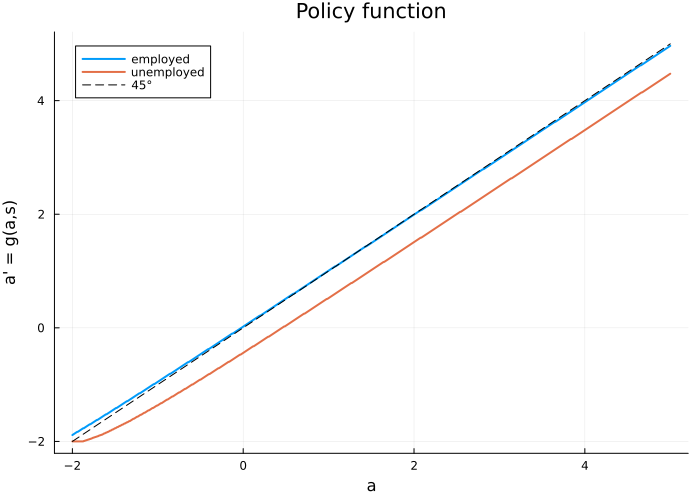
\includegraphics[width=0.7\textwidth]{policy_functions.png}
%   \caption{Policy function $g(a,s)$ for $s \in \{e, u\}$.}
% \end{figure}

\subsection*{4(b) Equilibrium bond price and wealth distribution}

% q* =

\subsection*{4(c) Lorenz curve and Gini}

% Wealth = earnings + net assets.


%==============================================================================
\section*{III. Welfare: incomplete vs.\ complete markets}
%==============================================================================

\[
  \lambda(a,s) = \left[
    \frac{W^{FB} + \frac{1}{(1-\alpha)(1-\beta)}}
         {v(a,s) + \frac{1}{(1-\alpha)(1-\beta)}}
  \right]^{\frac{1}{1-\alpha}} - 1
\]

\subsection*{(a) Consumption equivalents $\lambda(a,s)$}

\subsection*{(b) $W^{FB}$, $W^{INC}$, and $WG$}

\begin{table}[H]
  \centering
  \begin{tabular}{lc}
    \toprule
    & Value \\
    \midrule
    $W^{FB}$  & \\
    $W^{INC}$ & \\
    $WG$      & \\
    \bottomrule
  \end{tabular}
\end{table}

\subsection*{(c) Share favoring complete markets}

\end{document}
